% AIChipBench: State-Aware Evaluation of Coding Agents for AI Accelerators
% A coding agent writes kernels for an AI accelerator; evaluation checks the state at each stage.
\documentclass[tikz,border=0pt]{standalone}
% Shared look for the TikZ publication thumbnails.
% Canvas: 16cm x 10cm (16:10, matching the 640x400 WebP output), white, site palette.
% Labels are large (\lbl) because thumbnails are shown about 200px wide.
\usepackage[T1]{fontenc}
\usepackage{helvet}
\renewcommand{\familydefault}{\sfdefault}
\usepackage{amsmath,amssymb}
\usepackage{fontawesome5}
\usetikzlibrary{arrows.meta,calc,positioning,shapes.geometric,shapes.callouts,decorations.pathmorphing,shadows}

\definecolor{ink}{HTML}{2B2D42}
\definecolor{accent}{HTML}{B509AC}
\definecolor{teal}{HTML}{1E9BC0}
\definecolor{violet}{HTML}{6C5CE7}
\definecolor{orange}{HTML}{F28C28}
\definecolor{sun}{HTML}{F2C14E}
\definecolor{leaf}{HTML}{2CA58D}
\definecolor{alert}{HTML}{E5484D}
\definecolor{mist}{HTML}{EEF0F5}

\tikzset{
  every picture/.append style={line cap=round, line join=round},
  card/.style={rounded corners=10pt, draw=#1!75!black, line width=1.4pt, fill=#1!12},
  arrow/.style={-{Stealth[length=10pt,width=9pt]}, line width=2.2pt, draw=#1},
  soft shadow/.style={drop shadow={shadow xshift=0pt, shadow yshift=-3pt, opacity=0.18, fill=ink}},
  badge/.style={circle, fill=#1!14, draw=#1, line width=2pt, minimum size=2.3cm, text=#1},
}
\newcommand{\thumbcanvas}{\useasboundingbox[fill=white] (0,0) rectangle (16,10);}
\newcommand{\lbl}[1]{{\fontsize{20}{22}\selectfont\bfseries #1}}
\newcommand{\icon}[2][34]{{\fontsize{#1}{#1}\selectfont\faIcon{#2}}}
% Window chrome: dark editor panel with traffic-light dots. Args: x0, y0, x1, y1.
\newcommand{\editor}[4]{%
  \fill[ink, rounded corners=12pt, soft shadow] (#1,#2) rectangle (#3,#4);
  \foreach \c [count=\k] in {alert,sun,leaf} \fill[\c] ({#1+0.15+0.42*\k},{#4-0.42}) circle (0.13);
}

\begin{document}
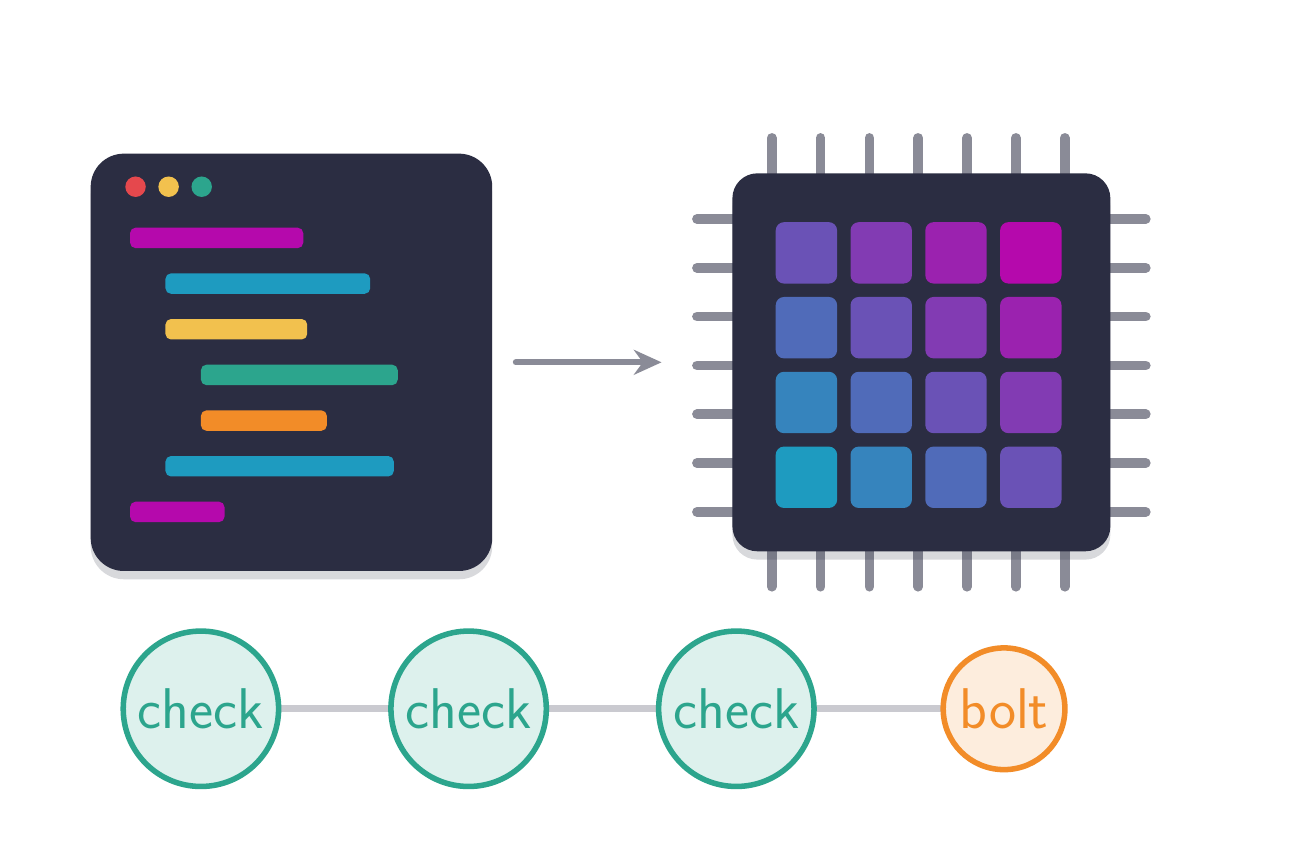
\begin{tikzpicture}
\thumbcanvas
% Agent-written kernel code.
\editor{0.8}{3.1}{5.9}{8.4}
\foreach \y/\x/\w/\c in {7.2/1.3/2.2/accent,6.62/1.75/2.6/teal,6.04/1.75/1.8/sun,5.46/2.2/2.5/leaf,
                        4.88/2.2/1.6/orange,4.3/1.75/2.9/teal,3.72/1.3/1.2/accent}
  \fill[\c, rounded corners=2pt] (\x,\y) rectangle ++(\w,0.26);
\draw[arrow=ink!55] (6.2,5.75) -- (8.05,5.75);
% Accelerator: a chip with a grid of compute tiles.
\foreach \i in {0,...,6} {
  \draw[ink!55, line width=3.5pt] ({9.45+\i*0.62},3.35) -- ++(0,-0.45) ({9.45+\i*0.62},8.15) -- ++(0,0.45);
  \draw[ink!55, line width=3.5pt] (8.95,{3.85+\i*0.62}) -- ++(-0.45,0) (13.75,{3.85+\i*0.62}) -- ++(0.45,0);
}
\fill[ink, rounded corners=9pt, soft shadow] (8.95,3.35) rectangle (13.75,8.15);
\foreach \i in {0,...,3} \foreach \j in {0,...,3} {
  \pgfmathtruncatemacro{\p}{(\i+\j)*100/6}
  \fill[accent!\p!teal, rounded corners=3pt] ({9.5+\i*0.95},{3.9+\j*0.95}) rectangle ++(0.78,0.78);
}
% State-aware evaluation: each stage is checked.
\draw[ink!25, line width=2.5pt] (2.2,1.35) -- (12.4,1.35);
\foreach \x/\ic/\c in {2.2/check/leaf,5.6/check/leaf,9.0/check/leaf,12.4/bolt/orange}
  \node[circle, fill=\c!16, draw=\c, line width=2pt, minimum size=1.1cm, text=\c] at (\x,1.35) {\icon[20]{\ic}};
\end{tikzpicture}
\end{document}
